\documentclass[12pt]{exam}
\usepackage[utf8]{inputenc}		% Caracteres latinos
\usepackage[spanish]{babel}		% Idioma español
\usepackage{geometry}			% Organizar el documento
\usepackage{graphicx}			% Incluir gráficos
\usepackage{makecell}			% Para personalizar las celdas de una tabla
\usepackage[nohdr]{mathexam}	% Añadimos el paquete mathexam (sin header)
\usepackage{amsmath}
\usepackage{amsfonts}
\usepackage{amssymb}
\usepackage{mathtools}
\usepackage{tikz,pgfplots}
\usepgfplotslibrary{polar}
\usepackage[shortlabels]{enumitem}
 \renewcommand{\baselinestretch}{1.5}
\usepackage{mathtools}
\usepackage{bm}
\usepackage{esvect}
\usepackage[fleqn]{mathtools}
\usepackage{relsize}
\usepackage{multirow}
\usepackage{multicol}
\usepackage[document]{ragged2e}
 \usepackage{textpos}
\usepackage{tcolorbox}
\usepackage{hyperref}




% Definimos la geometría de la primera página
\geometry{
	a4paper,                    % Tamaño del documento
	hmargin = {1.7cm, 1.7cm}, 	% Margen horizontal izquierdo, derecho
	vmargin = {1cm, 1cm},	    % Margen vertical superior, inferior
	headsep = 4mm,				% Separación entre el encabezado y el texto
	head = .2cm,				% Tamaño del encabezado
	% marginparsep = 5mm, 		% Seperación entre las notas y el texto
	% marginpar = 1.5cm,		% Tamaño de las notas
	includeall,                 % incluye el encabezado, footer y notas dentro del tamaño del documento
	nomarginpar,	            % Elimina las notas
	foot = 1cm,                 % Tamaño del footer
	twoside,                	% Habilita el modo de impresión a doble cara
}

\selectlanguage{spanish}        % Selecciona el idioma
\spanishdecimal{.}

%\pagestyle{headandfoot}         % Nuestro examen tendrá encabezado y pié

% DEFINIMOS EL ENCABEZADO
%\header{
%\begin{tabular}{l c c c l}
%            \makecell{\includegraphics[height=2.5cm]{logo.png}} &
%            \makecell{\textbf{IPEA 215} \\Raúl Scalabrini Ortiz} &
%            \makecell{Examen} &
%            \makecell{Curso\\1er Año} &
%             \makecell[l]{Apellido y %Nombre:\enspace\makebox[2in]{\hrulefill}\\Fecha: \today}
%        \end{tabular}}{}{}

% DEFINIMOS EL PIE
%\rfoot{Página \thepage\ de \numpages}
\newcommand{\iuni}{\pmb{\hat{\imath}}}
\newcommand{\juni}{\pmb{\hat{\jmath}}}
\newcommand{\kuni}{\pmb{\hat{k}}}
% DOCUMENTO
\begin{document}

\centering


\Large 
\textbf{\huge Tarea 1\\ \large Técnicas Cualitativa y Numérica}

\small
Fecha de entrega miércoles 13 de Octubre
\vskip10pt

\normalsize
\begin{tcolorbox}
\begin{itemize}
    \item SOLUCIONES SIN LOS DESARROLLOS CORRESPONDIENTES NO SE CONSIDERARÁ EL EJERCICIO.
    \item Resuelve 10 ejercicios en total: 3 de cada sección + 1 de cualquier sección.
    \item Por cada ejercicio extra a los 10 que resuelvas se te tomara como 1 punto sobre la calificación final.
    \item Si usas algún lenguaje de programación para resolver los ejercicios, por favor adjunta el código o el diagrama de flujo.
    \item Al final de tu tarea escribe la referencia de las páginas de internet si usaste alguna para visualizar las ecuaciones o sus soluciones.
\end{itemize}


\end{tcolorbox}
\pointpoints{punto}{puntos}
\pointformat{\bfseries\boldmath(\thepoints)}
\vskip10pt

    
    \begin{questions}
    
     \section{Campos direccionales}
    
     % 1 %
     \question
     De la ecuación diferencial $y'=x+\sen(y)$:
     \begin{enumerate}[a)]
         \item Una curva solución pasa por el punto $(1,\pi/2)$ ¿Cuál es su pendiente en ese punto?.
         \item Justifica porque para $x>1$ la soluciones son crecientes.
         \item Muestra que la concavidad de cada solución tiene por función $1+x\cos(y)+1/2\sen(2y)$. Justifica cada uno de los pasos.
         \item Una curva solución pasa por el punto $(0,0)$. Demuestra que la curva tiene un mínimo relativo en $(0,0)$.
     \end{enumerate}
    
     % 2 %
     \question
     De la ecuación diferencial $y'=x-y$ con valor inicial $y(0)=1$ y solución $\phi(x)$:
     \begin{enumerate}
         \item Demuestra que $\phi''(x)=1-\phi'(x)=1-x+\phi(x)$.
         \item Verifica que $y=x-1$ es una solución de $y'=x-y$ y explica porqué la gráfica de $\phi(x)$ siempre está por arriba de la recta $y=x-1$.
     \end{enumerate}
     
     % 3 %
     \question
     Traza las isoclinas y bosqueja varias curvas soluciones, incluyendo las curvas que satisfacen las condiciones iniciales dadas:
     \begin{enumerate}[a)]
         \item  $y'=ln|x|$, $y(1)=1$
         \item  $y'=1/x$, $y(-1)=1$
         \item  $y'=x+2y$, $y(0)=1$
         \item  $y'=x^2$, $y(0)=1$
     \end{enumerate}
        
     % 4 %
     \question
     Identifica la ecuación con su campo correspondiente. \textbf{Justifica} tu elección.
     
     \begin{tabular}{llll}
       i) $\frac{dy}{dx}=x-1$   & ii) $\frac{dy}{dx}=1-y^2$ & iii) $\frac{dy}{dx}=y^2-x^2$ & iv) $\frac{dy}{dx}=1-x$ \\
         v) $\frac{dy}{dx}=1-y$ & vi) $\frac{dy}{dx}=x^2-y^2$ & vii) $\frac{dy}{dx}=1+y$ & viii) $\frac{dy}{dx}=y^2-1$
     \end{tabular}
     
     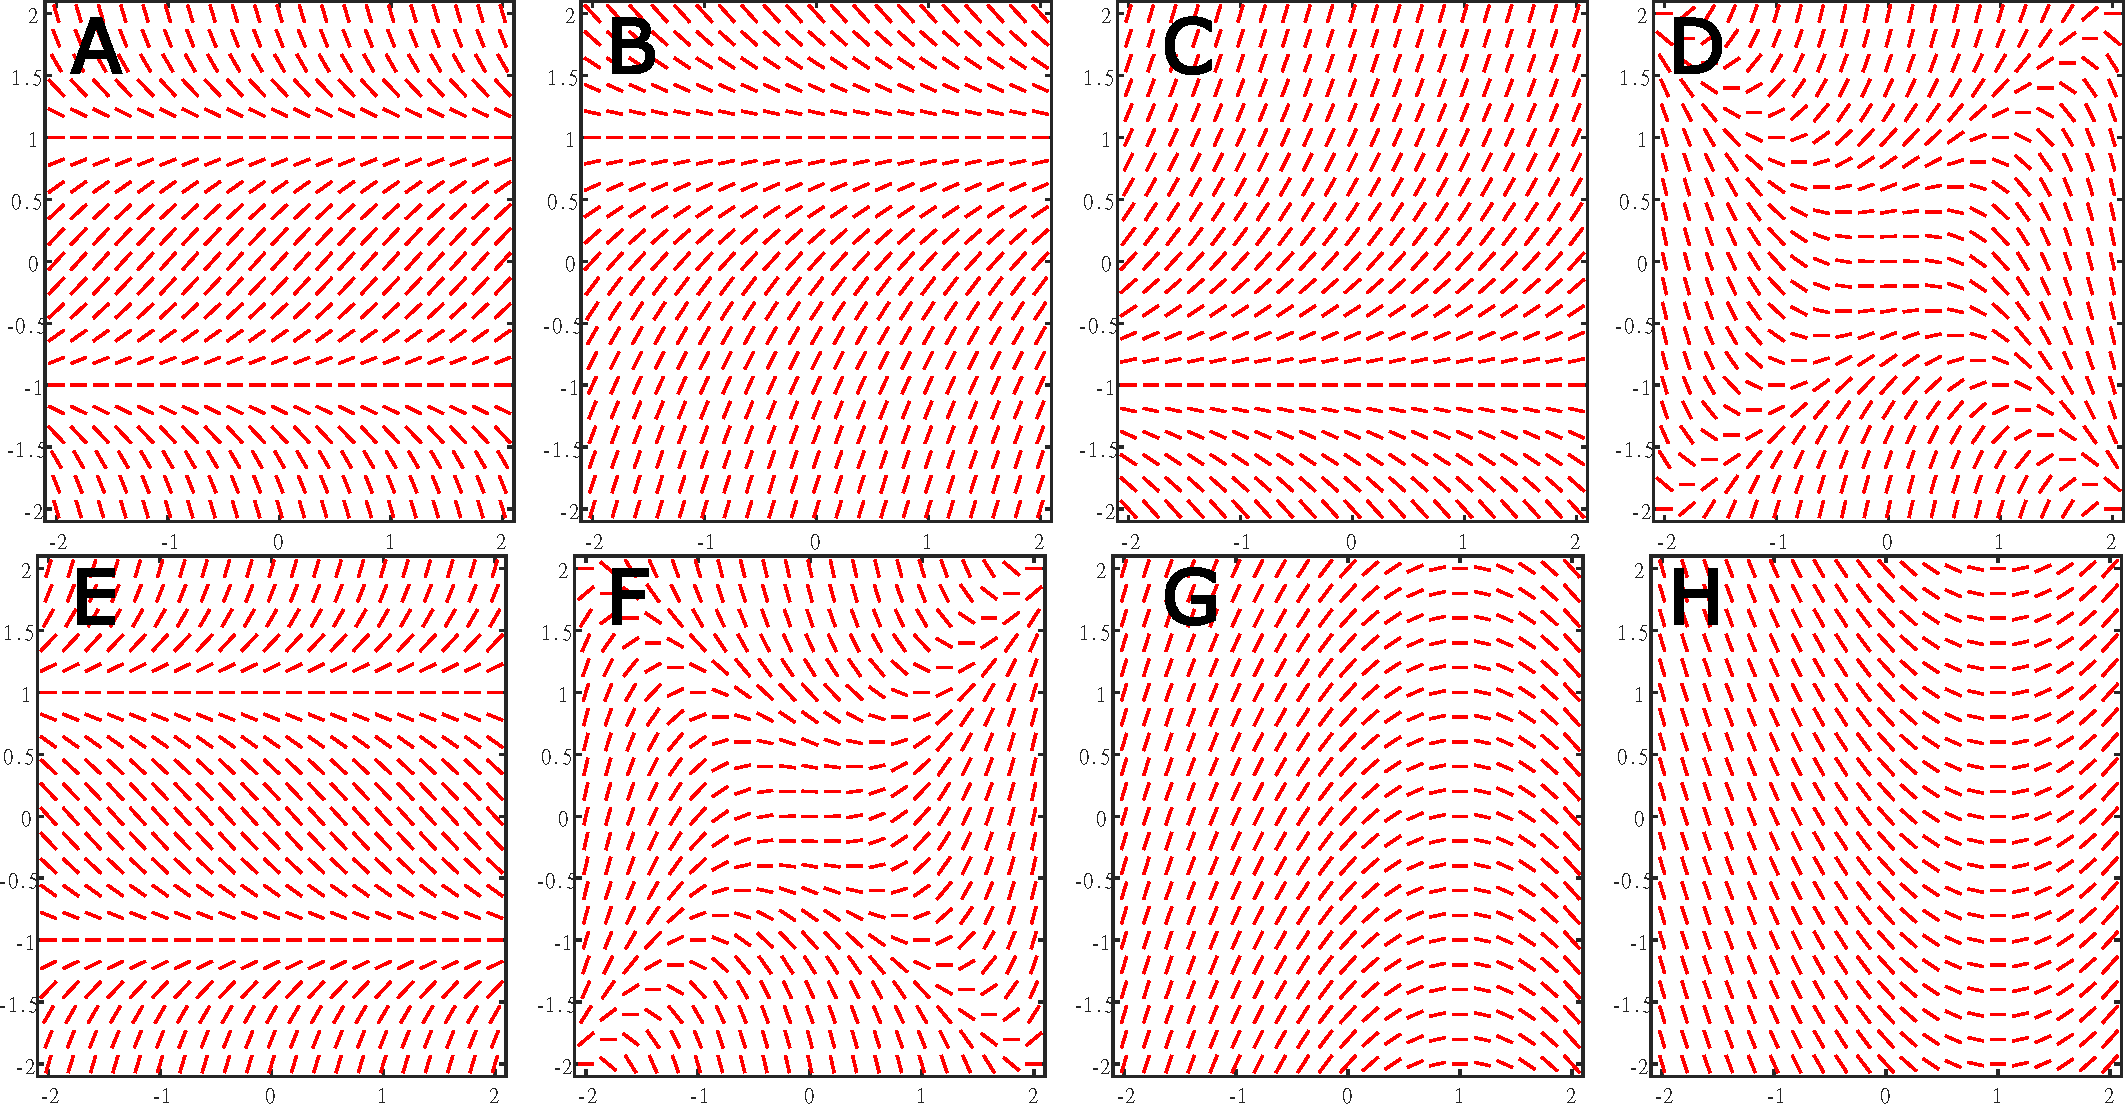
\includegraphics[scale=.48]{F1T1.pdf}


     % 5 %
     \question
     Considerando que $f(x,y)$ es continua y $f(x,3)=-1$ para toda x.
     \begin{enumerate}[a)]
         \item ¿Qué significa lo anterior si observamos el campo de pendientes de la ecuación diferencial $\frac{dy}{dx}=f(x,y)$?.
         \item ¿Qué puedes concluir sobre las soluciones $y(t)$ de $\frac{dy}{dx}=f(x,y)$? Por ejemplo, si $y(0)<3$ ¿puede $y(x)\rightarrow\infty$ cuando $x$ aumenta?
     \end{enumerate}

    \section{Método de Euler}

     % 6 %
     \question
     Aplica el método de Euler sobre las siguientes ecuaciones diferenciales con valor inicial y en el intervalo dado. Debes incluir: \textbf{a)} tabla y \textbf{b)} gráfica.
     
     \begin{enumerate}[a)]
         \item $\frac{dy}{dx}=y^2-4x$,\quad $y(0)=0.5$, \quad$0\leq x\leq2$, \quad$ \Delta x=0.25$.
         \item $\frac{dy}{dx}=e^{2/y}$, \quad$y(0)=2$, \quad$0\leq x\leq2$, \quad$\Delta x=0.5$
     \end{enumerate}

     % 7 %
     \question
     Utiliza el método de Euler para aproximar la solución de los siguientes problemas de valor inicial en los valores indicados, tomando los pasos 1, 2, 4 y 8:
     
     \begin{enumerate}[a)]
         \item $\frac{dy}{dx}=1-\sen(y)$,\quad $y(0)=0$. En $x=\pi$.
         \item $\frac{dx}{dt}=1+t\sen(tx)$, \quad$x(0)=0$. En $t=1$.
     \end{enumerate}

     % 8 %
     \question
     La ley de Stefan de la radiación establece que la tasa de cambio de temperatura de un cuerpo a $T(t)$ Kelvin en un medio a $M(t)$ Kelvin es proporcional a $M^4-T^4$. Es decir, $$\frac{dT}{dt}=K\left[M^4(t)-T^4(t) \right],$$ donde $K=2.9\times10^{-10}(\text{min})^{-1}$ y $M(t)=293$ Kelvin. Si $T(0)=360$ Kelvin, usa el método de Euler con $h=3\,\text{min}$ para aproximar la temperatura del cuerpo después de:
     
     \begin{enumerate}[a)]
         \item 30 minutos
         \item 60 minutos
     \end{enumerate}
% 9 %
     \question
     Considera la ecuación del circuito RC $$\frac{dv_c}{dt}=\frac{V(t)-v_c}{RC}.$$ Si el voltaje oscila periódicamente como $V(t)=2\cos(3t)$ con $R=4$ y $C=0.5$, usa el método de Euler para: \textbf{a) calcular} y \textbf{b) graficar} valores de las soluciones en el intervalo $0\leq t\leq10$ con las siguientes condiciones iniciales.
     
     \begin{enumerate}[a)]
         \item $v_c(0)=2$
         \item $v_c(0)=-2$
     \end{enumerate}

    \section{Línea Fase}

     % 10 %
     \question
     De las siguientes cuatro funciones $f(y)$, esboza la linea fase para la ecuación diferencial autónoma $dy/dt=f(y)$.
     \begin{center}
     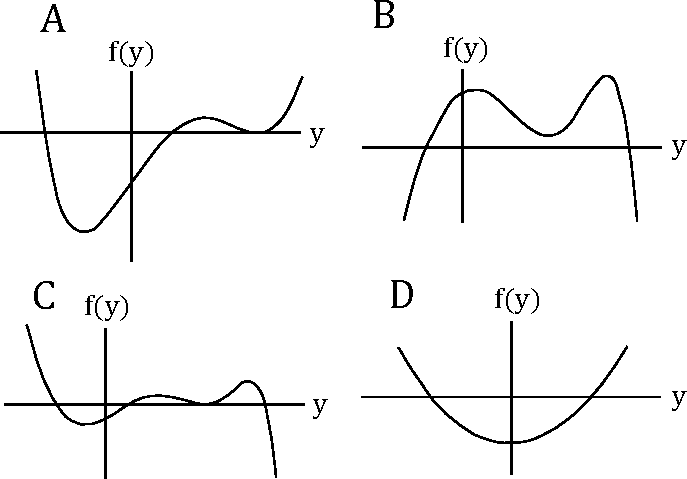
\includegraphics[scale=.8]{F2T1.pdf}
     \end{center}
     
     % 11 %
     \question
     De las siguientes líneas fases provenientes de ecuaciones autónomas $dy/dt=f(y)$, esboza la gráfica de la correspondiente función $f(y)$ asumiendo que $y=0$ es la mitad del segmento mostrado en cada caso.
     
     \begin{center}
     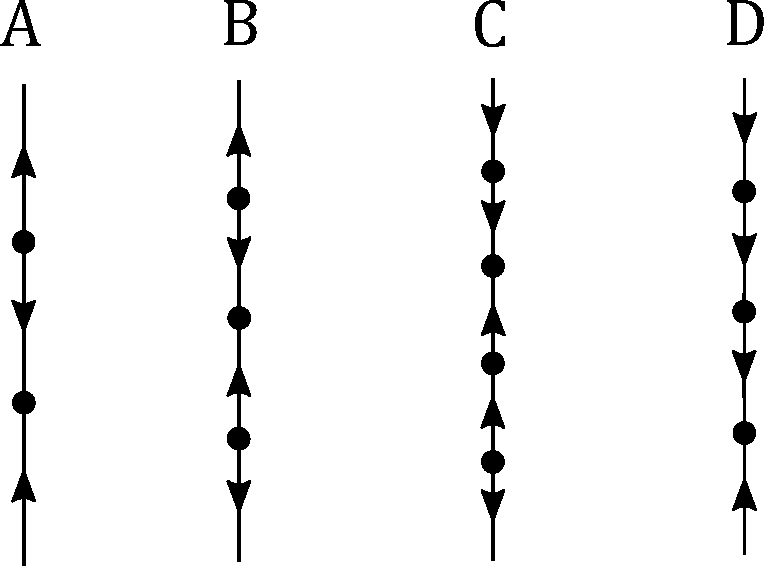
\includegraphics[scale=0.8]{F3T1.pdf}    
     \end{center}
     
     % 12 %
     \question
     El modelo de una cierta población esta descrito por una ecuación diferencial $dP/dt=f(P)$, donde $P(t)$ es la población al tiempo $t$ y de la cual se ha recabado la siguiente información:
     
     \begin{itemize}
         \item Se encontraron puntos de equilibrio solamente en $P=0$, $P=10$ y $P=50$.
         \item Cuando la población es igual a 100, ésta decrece.
         \item Cuando la población es igual a 25, ésta incrementa.
     \end{itemize}
     
     \begin{enumerate}[a)]
         \item Esboza las dos posibles líneas fases del sistema para $P>0$.
         \item Esboza las correspondientes funciones $f(P)$ para cada una de las líneas fase.
         \item Da una fórmula para la función $f(P)$ cuyas gráficas coincidan \textbf{cualitativamente} con las gráficas de \textbf{b)} para cada una de las líneas fase.
     \end{enumerate}


     % 13 %
     \question
     Supón que $dy/dt=f(y)$ tiene un punto de equilibrio en $y=y_0$ y
     
     \begin{enumerate}[a)]
         \item $f'(y_0)=0$, $f''(y_0)=0$ y $f'''(y_0)>0$: ¿$y_0$ es una fuente, un sumidero o un nodo?
         \item $f'(y_0)=0$, $f''(y_0)=0$ y $f'''(y_0)<0$: ¿$y_0$ es una fuente, un sumidero o un nodo?
         \item $f'(y_0)=0$ y $f''(y_0)>0$: ¿$y_0$ es una fuente, un sumidero o un nodo?
     \end{enumerate}



     

        \end{questions}
%         \vskip30pt
%  \RaggedRight
%  PUNTO EXTRA


    
    \newpage


\runningfooter{}{}{Página \thepage\ de \numpages}



\end{document}
